\documentclass[a4paper,11pt,oneside]{memoir}

% Castellano
\usepackage[spanish]{babel}
\selectlanguage{spanish}
\usepackage[utf8]{inputenc}
\usepackage{placeins}
\usepackage{caption}
\usepackage{subcaption}
\usepackage[linesnumbered,ruled,vlined,spanish]{algorithm2e}


\RequirePackage{booktabs}
\RequirePackage[table]{xcolor}
\RequirePackage{xtab}
\RequirePackage{multirow}

% Links
\usepackage[colorlinks]{hyperref}
\hypersetup{
	allcolors = {red}
}

% Ecuaciones
\usepackage{amsmath}

% Rutas de fichero / paquete
\newcommand{\ruta}[1]{{\sffamily #1}}

% Párrafos
\nonzeroparskip


% Imagenes
\usepackage{graphicx}
\newcommand{\imagen}[2]{
	\begin{figure}[!h]
		\centering
		\includegraphics[width=0.9\textwidth]{#1}
		\caption{#2}\label{fig:#1}
	\end{figure}
	\FloatBarrier
}

\newcommand{\imagenflotante}[2]{
	\begin{figure}%[!h]
		\centering
		\includegraphics[width=0.9\textwidth]{#1}
		\caption{#2}\label{fig:#1}
	\end{figure}
}



% El comando \figura nos permite insertar figuras comodamente, y utilizando
% siempre el mismo formato. Los parametros son:
% 1 -> Porcentaje del ancho de página que ocupará la figura (de 0 a 1)
% 2 --> Fichero de la imagen
% 3 --> Texto a pie de imagen
% 4 --> Etiqueta (label) para referencias
% 5 --> Opciones que queramos pasarle al \includegraphics
% 6 --> Opciones de posicionamiento a pasarle a \begin{figure}
\newcommand{\figuraConPosicion}[6]{%
  \setlength{\anchoFloat}{#1\textwidth}%
  \addtolength{\anchoFloat}{-4\fboxsep}%
  \setlength{\anchoFigura}{\anchoFloat}%
  \begin{figure}[#6]
    \begin{center}%
      \Ovalbox{%
        \begin{minipage}{\anchoFloat}%
          \begin{center}%
            \includegraphics[width=\anchoFigura,#5]{#2}%
            \caption{#3}%
            \label{#4}%
          \end{center}%
        \end{minipage}
      }%
    \end{center}%
  \end{figure}%
}

%
% Comando para incluir imágenes en formato apaisado (sin marco).
\newcommand{\figuraApaisadaSinMarco}[5]{%
  \begin{figure}%
    \begin{center}%
    \includegraphics[angle=90,height=#1\textheight,#5]{#2}%
    \caption{#3}%
    \label{#4}%
    \end{center}%
  \end{figure}%
}
% Para las tablas
\newcommand{\otoprule}{\midrule [\heavyrulewidth]}
%
% Nuevo comando para tablas pequeñas (menos de una página).
\newcommand{\tablaSmall}[5]{%
 \begin{table}
  \begin{center}
   \rowcolors {2}{gray!35}{}
   \begin{tabular}{#2}
    \toprule
    #4
    \otoprule
    #5
    \bottomrule
   \end{tabular}
   \caption{#1}
   \label{tabla:#3}
  \end{center}
 \end{table}
}

%
% Nuevo comando para tablas pequeñas (menos de una página).
\newcommand{\tablaSmallSinColores}[5]{%
 \begin{table}[H]
  \begin{center}
   \begin{tabular}{#2}
    \toprule
    #4
    \otoprule
    #5
    \bottomrule
   \end{tabular}
   \caption{#1}
   \label{tabla:#3}
  \end{center}
 \end{table}
}

\newcommand{\tablaApaisadaSmall}[5]{%
\begin{landscape}
  \begin{table}
   \begin{center}
    \rowcolors {2}{gray!35}{}
    \begin{tabular}{#2}
     \toprule
     #4
     \otoprule
     #5
     \bottomrule
    \end{tabular}
    \caption{#1}
    \label{tabla:#3}
   \end{center}
  \end{table}
\end{landscape}
}

%
% Nuevo comando para tablas grandes con cabecera y filas alternas coloreadas en gris.
\newcommand{\tabla}[6]{%
  \begin{center}
    \tablefirsthead{
      \toprule
      #5
      \otoprule
    }
    \tablehead{
      \multicolumn{#3}{l}{\small\sl continúa desde la página anterior}\\
      \toprule
      #5
      \otoprule
    }
    \tabletail{
      \hline
      \multicolumn{#3}{r}{\small\sl continúa en la página siguiente}\\
    }
    \tablelasttail{
      \hline
    }
    \bottomcaption{#1}
    \rowcolors {2}{gray!35}{}
    \begin{xtabular}{#2}
      #6
      \bottomrule
    \end{xtabular}
    \label{tabla:#4}
  \end{center}
}

%
% Nuevo comando para tablas grandes con cabecera.
\newcommand{\tablaSinColores}[6]{%
  \begin{center}
    \tablefirsthead{
      \toprule
      #5
      \otoprule
    }
    \tablehead{
      \multicolumn{#3}{l}{\small\sl continúa desde la página anterior}\\
      \toprule
      #5
      \otoprule
    }
    \tabletail{
      \hline
      \multicolumn{#3}{r}{\small\sl continúa en la página siguiente}\\
    }
    \tablelasttail{
      \hline
    }
    \bottomcaption{#1}
    \begin{xtabular}{#2}
      #6
      \bottomrule
    \end{xtabular}
    \label{tabla:#4}
  \end{center}
}

%
% Nuevo comando para tablas grandes sin cabecera.
\newcommand{\tablaSinCabecera}[5]{%
  \begin{center}
    \tablefirsthead{
      \toprule
    }
    \tablehead{
      \multicolumn{#3}{l}{\small\sl continúa desde la página anterior}\\
      \hline
    }
    \tabletail{
      \hline
      \multicolumn{#3}{r}{\small\sl continúa en la página siguiente}\\
    }
    \tablelasttail{
      \hline
    }
    \bottomcaption{#1}
  \begin{xtabular}{#2}
    #5
   \bottomrule
  \end{xtabular}
  \label{tabla:#4}
  \end{center}
}



\definecolor{cgoLight}{HTML}{EEEEEE}
\definecolor{cgoExtralight}{HTML}{FFFFFF}

%
% Nuevo comando para tablas grandes sin cabecera.
\newcommand{\tablaSinCabeceraConBandas}[5]{%
  \begin{center}
    \tablefirsthead{
      \toprule
    }
    \tablehead{
      \multicolumn{#3}{l}{\small\sl continúa desde la página anterior}\\
      \hline
    }
    \tabletail{
      \hline
      \multicolumn{#3}{r}{\small\sl continúa en la página siguiente}\\
    }
    \tablelasttail{
      \hline
    }
    \bottomcaption{#1}
    \rowcolors[]{1}{cgoExtralight}{cgoLight}

  \begin{xtabular}{#2}
    #5
   \bottomrule
  \end{xtabular}
  \label{tabla:#4}
  \end{center}
}


















\graphicspath{ {./img/} }

% Capítulos
\chapterstyle{bianchi}
\newcommand{\capitulo}[2]{
	\setcounter{chapter}{#1}
	\setcounter{section}{0}
	\chapter*{#2}
	\addcontentsline{toc}{chapter}{#2}
	\markboth{#2}{#2}
}

% Apéndices
\renewcommand{\appendixname}{Apéndice}
\renewcommand*\cftappendixname{\appendixname}

\newcommand{\apendice}[1]{
	%\renewcommand{\thechapter}{A}
	\chapter{#1}
}

\renewcommand*\cftappendixname{\appendixname\ }

% Formato de portada
\makeatletter
\usepackage{xcolor}
\newcommand{\tutor}[1]{\def\@tutor{#1}}
\newcommand{\course}[1]{\def\@course{#1}}
\definecolor{cpardoBox}{HTML}{E6E6FF}
\def\maketitle{
  \null
  \thispagestyle{empty}
  % Cabecera ----------------
\noindent
\includegraphics[width=\textwidth]{cabecera}\vspace{1cm}%
  \vfill
  % Título proyecto y escudo informática ----------------
  \colorbox{cpardoBox}{%
    \begin{minipage}{.8\textwidth}
      \vspace{.5cm}\Large
      \begin{center}
      \textbf{TFG del Grado en Ingeniería Informática}\vspace{.6cm}\\
      \textbf{\LARGE\@title{}}
      \end{center}
      \vspace{.2cm}
    \end{minipage}

  }%
  \hfill\begin{minipage}{.20\textwidth}
    
\includegraphics[width=\textwidth]{escudoInfor}
  \end{minipage}
  \vfill
  % Datos de alumno, curso y tutores ------------------
  \begin{center}%
  {%
    \noindent\LARGE
    Presentado por \@author{}\\ 
    en Universidad de Burgos --- \@date{}\\
    Tutor: \@tutor{}\\
  }%
  \end{center}%
  \null
  \cleardoublepage
  }
\makeatother

\newcommand{\nombre}{Nombre del alumno} %%% cambio de comando

% Datos de portada
\title{título del TFG}
\author{\nombre}
\tutor{nombre tutor}
\date{\today}

\begin{document}

\maketitle



\null\cleardoublepage


%%%%%%%%%%%%%%%%%%%%%%%%%%%%%%%%%%%%%%%%%%%%%%%%%%%%%%%%%%%%%%%%%%%%%%%%%%%%%%%%%%%%%%%%
\pagestyle{empty}


\noindent
\includegraphics[width=\textwidth]{cabecera}\vspace{1cm}

\noindent D. nombre tutor, profesor del departamento de nombre departamento, área de nombre área.

\noindent Expone:

\noindent Que el alumno D. \nombre, con DNI dni, ha realizado el Trabajo final de Grado en Ingeniería Informática titulado título de TFG. 

\noindent Y que dicho trabajo ha sido realizado por el alumno bajo la dirección del que suscribe, en virtud de lo cual se autoriza su presentación y defensa.

\begin{center} %\large
En Burgos, {\large \today}
\end{center}

\vfill\vfill\vfill

% Author and supervisor
\begin{minipage}{0.45\textwidth}
\begin{flushleft} %\large
Vº. Bº. del Tutor:\\[2cm]
D. nombre tutor
\end{flushleft}
\end{minipage}
\hfill
\begin{minipage}{0.45\textwidth}
\begin{flushleft} %\large
Vº. Bº. del co-tutor:\\[2cm]
D. nombre co-tutor
\end{flushleft}
\end{minipage}
\hfill

\vfill

% para casos con solo un tutor comentar lo anterior
% y descomentar lo siguiente
%Vº. Bº. del Tutor:\\[2cm]
%D. nombre tutor


\null\cleardoublepage
\null\cleardoublepage




\frontmatter

% Abstract en castellano
\renewcommand*\abstractname{Resumen}
\begin{abstract}
En este primer apartado se hace una \textbf{breve} presentación del tema que se aborda en el proyecto.
\end{abstract}

\renewcommand*\abstractname{Descriptores}
\begin{abstract}
Palabras separadas por comas que identifiquen el contenido del proyecto Ej: servidor web, buscador de vuelos, android \ldots
\end{abstract}

\clearpage

% Abstract en inglés
\renewcommand*\abstractname{Abstract}
\begin{abstract}
A \textbf{brief} presentation of the topic addressed in the project.
\end{abstract}

\renewcommand*\abstractname{Keywords}
\begin{abstract}
keywords separated by commas.
\end{abstract}

\clearpage

% Indices
\tableofcontents

\clearpage

\listoffigures

\clearpage

%\listoftables

%\clearpage

\mainmatter
\newcommand{\grad}{$^{\circ}$}
\capitulo{1}{Introducción}
%\maketitle
Este proyecto es un trabajo que se hara en colaboracion con el Laboratorio de Evolucion Humana \url{http://www3.ubu.es/atapuerca/index.html}, del departamento de Ciencias Históricas de la Universidad de Burgos, concretamente la colaboradora del proyecto sera la Dra. Rebeca García González \cite{ubu:Rebe},  que estudia paleobiología y paleoecología de homínidos en la Universidad de Burgos, 

El problema planteado, que se quiere automatizar, consiste en crear una herramienta o aplicación para detectar las estrías que se producen en los dientes, al masticar distintos tipos de comida, tal y como se explica en el paper en el que nos basaremos el método \cite{garcia2015dietary}.

Para ser mas exactos, todos los materiales tienen una dureza tangible, los dientes tienen una dureza superior a la de los alimentos, sin embargo  algunas partes de los alimentos tienen mas dureza que los dientes, por lo que los consiguen rallar, creando unas estrías que dependiendo de los alimentos siguen distintos patrones.

 
Vamos a detectar esas estrías, pero en el contexto de la prehistoria, para después poder clasificar los individuos en función de la dieta que llevaban, la forma de clasificacion en las direcciones esta determinada por el paper \cite{garcia2015dietary}, en el que nos indican los ángulos de clasificación para las 4 direcciones:
\begin{itemize}
\item Horizontales <<H>>: Con ángulos comprendidos entre 0\grad a 22.5\grad y 157.5\grad a 180\grad.
\item Verticales <<V>>: Con ángulos comprendidos entre 67.5\grad a 112.5\grad. 
\item Disto-occlusal a mesio-cervical <<DM>>: Con ángulos comprendidos entre 112.5\grad a 157.5\grad.
\item Mesio-occlusal a disto-cervical <<MD>>: Con ángulos comprendidos entre 22.5\grad a 67.5\grad.
\end{itemize}
Para mas tarde extrapolar los datos de estas orientaciones y proyectar un punto en un plano de dos dimensiones, que nos indicara a que región pertenece dicho individuo, esto podra ser estimado por las dos funciones que propone Lalueza en su paper \cite{Lalueza:perez}. 


Nuestro proyecto va a tener una parte de visión artificial, que detecte las lineas que han pintado, sobre las imágenes de microscopio de electrones a 100 aumentos, otra parte de diseño e implementación, del software a usar y distintos análisis de las herramientas que usaremos para ello.

La herramienta a usar tendrá implementados 3 modos claramente diferenciados.

\begin{itemize}
\item Modo semi-automático: detección, conteo y análisis de las lineas pintadas sobre una imagen.
\item Pintar lineas manualmente sobre la imagen o corregir las posibles lineas que el anterior modo no consiga detectar.
\item Automático que buscara las estrías por la imagen. Este modo quedara como extra, ya que hemos tenido una gran agilidad realizando el proyecto, vamos a tratar esta parte para completar e investigar sobre detección automática de bordes.
\end{itemize}








 
\capitulo{2}{Objetivos del proyecto}

Este apartado explica de forma precisa y concisa cuales son los objetivos que se persiguen con la realización del proyecto. Se puede distinguir entre los objetivos marcados por los requisitos del software a construir y los objetivos de carácter técnico que plantea a la hora de llevar a la práctica el proyecto.

\section{Objetivos}
Esta parte se corresponde con el esquema de todos los puntos.
\begin{itemize}
\item Analizar el problema planteado por Rebeca, nuestra colaboradora del Laboratorio de Evolución Humana, y buscar una solución:
	\begin{itemize}
		\item Primero tenemos que documentarnos y saber que son las líneas a detectar.
		\item Buscar una solución para detectar dichas estrías pintadas, de forma automática, ya que hasta ahora era un problema manual que tenían que medir a mano.
		\item Permitir que se pinten através de la aplicación para futuras imágenes.
		\item Iniciar la forma de detección completamente automática.
	\end{itemize}
\item Crear un notebook para el procesado:
	\begin{itemize}
		\item Crear un prototipo interactivo atrevés de los notebooks de jupyter.
		\item Procesar la imagen para obtener la mascara o imagen binarizada con las líneas.
		\item Detectar los segmentos que se corresponden con las líneas.
		\item Juntar los segmentos para obtener líneas reales.
	\end{itemize}
\item Crear la aplicación:
	\begin{description}
		\item Crear una interfaz gráfica con la imagen, y botonería.
		\item [Modo 1] Modo semi-automátic, detección, conteo y análisis de estrías.
		\item [Modo 2] Permitir pintar estrías y corrección de segmentos.
		\item [Modo 3] Completamente automático.
	\end{description}
\end{itemize}

\section{Resumen}

El problema va a consistir en detectar las líneas que tienen ya pintadas y detectar desde cero las sin pintar, en las imágenes, para poder automatizar dicho proceso, ya que los pasos anteriores eran:
\begin{itemize}
\item Pintar las estrías encima de la imagen.
\item Obtener de las estrías, de forma manual, su tamaño, ángulo, dirección.
\end{itemize}
Y los pasos a través de nuestra aplicación son:
\begin{itemize}
\item Abrir la imagen y seleccionar el color de las líneas
\item Dar al botón de calcular las líneas y guardarlo: Tendíamos el CSV con los estadísticos y atributos de ellas.
\end{itemize}
Como podemos observar, nuestros pasos nos devuelven las estrías de forma mucho mas cómoda y mas rápida que buscándolas a mano.

\subsection{Crear un prototipo} 
En esta parte hemos pensado que sería mas cómodo, antes de ponernos a diseñar o implementar, comprobar que lo que tenemos pensado para resolver el problema que funcione.

Crear un Notebook de Jupyter \ref{notebook:jupiter} no nos exige que programemos nada de la GUI, al ser interactivo, se va a implementar todos los pasos necesarios para resolver el problema y una vez conseguido. Como producto tenemos el núcleo de cálculo y pasamos a hacer el diseño.

\subsection{Crear la aplicación}
Llegados a este punto ya tendremos todo lo necesario para hacer nuestras clases y nuestra aplicación.

Así que ya tenemos todo lo necesario y solo queda el producto entregable que sera la aplicación enlazada con la GUI junto con, la creación de botones, pestañas, ventanas con sus respectivas implementaciones y funcionalidades.
\capitulo{3}{Conceptos teóricos}
En esta sección vamos a centrarnos en explicar todos los conceptos necesarios para poder entender los pasos de los procesos realizados en la aplicación y saber en que se sustentan.

\begin{itemize}
\item Espacios de color: Las imágenes nos son mas que matrices de numeros que expresan, valores o poderaciones, distintos para representar los colores. La suma de todas ellas transmitido atrabes de un medio de reproducion, pantalla o similar, nos muestran las imagenes.
Cada espacio de color tiene unas propiedades y unas ventajas. Para obtener las característica que buscamos, con mayor o menor dificultad, por eso es necesario explicar los distintos espacios de colores.

\item Preprocesados:
Estos se compondrán de una serie de pasos previos a la obtención de los segmentos correspondientes a las estrías.
	\begin{itemize}
		\item La reducción de grosor: Es un paso clave en el procesado porque gracias a esto obtenemos los resultados que mas se ajustan a la realidad.
No es complejo pero si que es muy útil y sin este paso no serviría nada, nuestro procesado, (su función es eliminar el ruido).
		\item Bordes: Al final las estrías que detectamos no son mas que bordes dentro de la imagen y todo lo usado es para su detección, por lo que es necesaria su explicación. Como dato curioso, para la resolución de nuestro problema lo que hemos hecho es reducirlo a un problema de detección de bordes.
	\end{itemize}

\item Análisis: 
Una vez que tengamos la máscara sobre la que detectar las características que estamos buscando, (este proceso tampoco sera directo), por lo que tendremos que hacer una serie de pasos, para obtener nuestro objetivo.
	\begin{itemize}
	\item Transformada de Hough: Es un procedimiento matemático para buscar segmentos dentro de las imágenes binarizadas, dado que es complejo, es necesario explicar porque funciona y en que consiste.

	\item Grafos: Gracias a la teoría de grafos podemos procesar muchos segmentos similares en uno solo, de forma sencilla y eficiente, por lo que es necesaria su explicación.
	\end{itemize}

\end{itemize}



\section{Espacios de color }
El color que percibimos en los objetos que nos rodean depende de la radiación reflejada en ellos. Según los estudios, nosotros como humanos tenemos un rango <<de luz visible>>, ese rango son en verdad tres frecuencias diferentes dentro del rango 769THz a 384THz~\cite{Manual:HAE}.
Por lo que en verdad una imagen que percibimos es la unión de las tres frecuencias diferentes y para poder simular este hecho las maquinas simulan esta capacidad innata de los humanos creando los espacios de color que son modelos matemáticos para representar en una maquina lo que se observa en la figura \ref{fig:3.1}.

\begin{figure}[h]
\centering
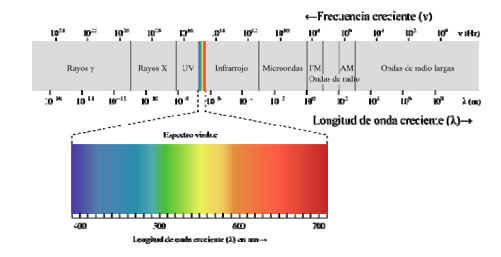
\includegraphics[width=.9\textwidth]{EspacioDeColor}
\caption{Frecuencias de luz visible \cite{Manual:HAE}}
\label{fig:3.1}
\end{figure}

\subsection{RGB}
El modelo RGB es usado por todos los sistemas digitales para la representación y captura de imágenes.

Se divide en tres canales como se muestra en la figura \ref{fig:3.2}.

\begin{itemize}
	\item R: canal del rojo (RED) contiene la intensidad de rojo de cada pixel
	\item G: canal del verde (GREEN) contiene la intensidad de verde de cada pixel
	\item B: canal del azul (BLUE) contiene la intensidad de azul de cada pixel
\end{itemize}

\begin{figure}[h]
\centering
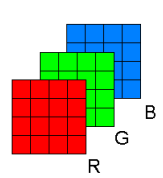
\includegraphics[width=.3\textwidth]{RGB_Canales}
\caption{Los tres canales del espacio RGB~\cite{Manual:HAE}}
\label{fig:3.2}
\end{figure}
La combinación de estos colores crea todas la gama de colores representable.
El valor de la intensidad de cada canal depende de la codificación usada para su representación (Ocho bits dan dieciséis millones de colores) como se muestra en la figura  \ref{fig:3.3}.

\begin{figure}[h]
\centering
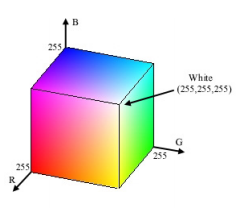
\includegraphics[width=.3\textwidth]{RGB}
\caption{Representación del modelo RGB~\cite{Manual:HAE}}
\label{fig:3.3}
\end{figure}

\subsection{HSV}
El modelo HSV \cite{modelo:hsv} esta orientado a la descripción de los colores en términos mas prácticos para el ser humano que el RGB, los canales significan algo mas que la cantidad de cada color, por lo que es mas practico para el ser humano. (Lo que se observa en la figura \ref{fig:3.4}).
 
\begin{itemize}
	\item H: (Matiz) que representa el tono o color.
	\item S: (Saturación) representa el nivel de saturación de un color.
	\item V: (Brillo) representa la intensidad lumínica.
\end{itemize}

\begin{figure}[h]
\centering
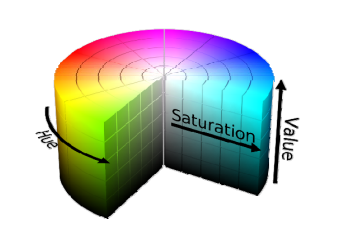
\includegraphics[width=.35\textwidth]{HSV}
\caption{Representación del modelo HSV~\cite{Manual:HAE}}
\label{fig:3.4}
\end{figure}

Una ventaja con otros espacios de color parecidos es que este permite representar todas las combinaciones del espacio RGB.
Pero su característica principal es que el canal de saturación, (representa la viveza de un color) nos permitirá diferenciar las estrías del resto. Al seleccionar el color de las estrías pintadas, entre grises que tendrán saturación muy baja y el color pintado sobre estas.

\subsection{CIELAB}
El modelo lab \cite{wiki:lab},mas conocido como CIELAB, es otra forma de representar los colores. Este en concreto, se basa en como representa los colores el ojo humano, la diferencia entre LAB y CIELAB, es que CIELAB utiliza raíces cubicas, mientras que LAB usa raíces cuadradas.

El modelo lo podemos ver en la siguiente figura  \ref{fig:3.8}.

\begin{figure}[h]
\centering
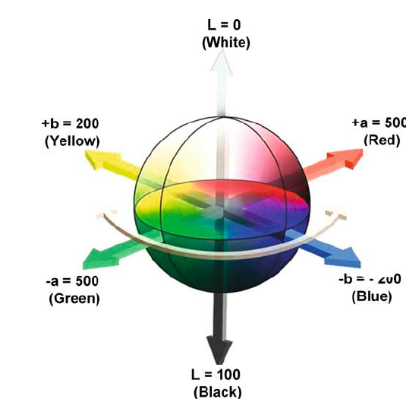
\includegraphics[width=.35\textwidth]{CieLAB}
\caption{Representación del modelo CIELAB~\cite{cie:LAB}}
\label{fig:3.8}
\end{figure}


Componentes del modelo:
\begin{itemize}
	\item L: Luminosidad de negro a blanco.
	\item A: Desde el color rojo al verde.
	\item B: Es la gradiente del color azul.
\end{itemize}

Ventajas:
\begin{itemize}
\item Corregir colores: Es mas rápido hacer una corrección del color que en otros espacios de color.
\item Mas cantidad de colores: Con esta representación del color conseguimos representar mayor numero de colores, incluso colores imaginarios \footnote{Estos son colores que no es capaz de detectar el ojo humano, principalmente se usa para manipulación de imágenes.}.
\item La perdida es mínima al cambiar a otro espacio de color.
\end{itemize}

El uso de este espacio de color viene dado por la necesidad de calcular la distancia a otros colores, que en este caso la diferencia. Caracteriza mejor que los demás espacios y por esto vamos a usar este espacio.
\section{Transformada de Hough }

Uno de los puntos relevantes del proyecto es la detección de las líneas pintadas o detectadas por el algoritmo (modo automático) para ello vamos a usar una técnica que sirve para detectar formas, expresadas de forma matemática, dentro de imágenes.

Esta técnica fue inventada por Richard Duda y Peter Hart en 1972 pero diez años antes, Paul Hough propuso y patentó \cite{pat:patHough} la idea inicial de detectar líneas en la imagen. Mas tarde se generalizó para detectar cualquier figura.

\subsection{Teoría}

Normalmente para detectar figuras sencillas en una imagen primero hay que usar algún algoritmo de detección de bordes o una binarización de la imagen, quedándonos con la región de interés apropiada (los píxeles que forman las rectas) pero normalmente faltan píxeles por el ruido en la imagen.

Para ello el método de Hough propone solucionar el problema detectando grupos de puntos que forman los bordes de la misma figura y así conseguir unirlos creando la recta real a la que pertenecen. Como podemos ver en el siguiente pseudocódigo 
\ref{alg:Hough}.

\label{alg:Hough}
%Hough
\begin{algorithm*}
\caption{Pseudocódigo de la transformada}
\DontPrintSemicolon
\KwIn{Imagen}
\KwOut{(list) de segmentos encontrados }

%$ S = \varnothing $

\ForEach {punto en la imagen}{
		\If {punto \textbf{(x,y)} esta en un borde:}{
			\ForEach {angulo en ángulos $\Theta$ }{
				Calcular $\rho$  para el punto (x,y) con angulo $\Theta$ \;
				Incrementar la posición ($\rho$ , $\Theta$ ) en el acumulador\;
			}
		}
}
Buscar las posiciones con mayores valores en el acumulador\;	

\Return {$rectas$ Las rectas cuyos valores son los mayores en el acumulador}
\end{algorithm*}

\subsection{Limitaciones}
Para que este proceso sea exitoso, los bordes del objeto deben ser detectados correctamente con un buen pre-procesado de la imagen y aparecer claramente las nubes de puntos que forman las rectas.
Como se muestra en el figura \ref{fig:3.5}.

\begin{figure}[h]
\centering
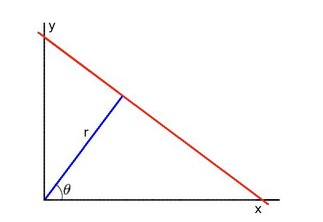
\includegraphics[width=.3\textwidth]{hough}
\caption{Líneas de Hough~\cite{opencv:HoughIm}}
\label{fig:3.5}
\end{figure}
\subsection{Transformada probabilística de Hough}

Tal y como se explica en \cite{Kiryati20001157}, la transformada probabilística de Hough es una version que se basa en que la detección de bordes o la producción de la imagen binaria, que contiene el objeto. Podría tener ruido y por lo tanto los píxeles, correspondientes al ruido en la transformada normal podrían ser considerados, una recta. Cuando en verdad es ruido.

Para que unos puntos sean considerados recta en la transformada probabilística, es necesario menos puntos que en la transformada normal de Hough.
Pero este método penaliza a los puntos que se encuentran aleatoriamente por toda la imagen (ruido), frente a los que se localizan perfectamente agrupados formando las rectas. 
Un exceso de ruido en la imagen también haría este método inservible, pero para pequeñas cantidades lo hacen mas preciso que el método normal.
Otra ventaja es que con este método obtenemos el segmento que necesitamos, no la prolongación de él hasta el infinito.

\section{Reducción de grosor: Skeletonize}
Tal y como se explica en \cite{scik:skeleton}, dentro del pre-procesado de la imagen, uno de los puntos clave, como se explica en el párrafo siguiente, para que nuestro método funcione.

Después de su binarización y la detección de los bordes de la imagen a procesar, debemos reducir la región sobre la que aplicar la transformada de Hough, así conseguiremos que esta sea mas rápida, y detecte menor número de líneas imaginarias por cada línea real.

Esto lo conseguiremos usando una función de esqueletonizado que nos devuelve lo que su nombre indica: el esqueleto de los bordes de la imagen reducidos a un pixel. Como podemos observar en la imagen \ref{fig:3.6}.


\begin{figure}
\begin{subfigure}[b]{.5\linewidth}
\centering\large 
\includegraphics[width=.9\textwidth]{skeletonizeA}
\caption{Original}
\end{subfigure}%
\begin{subfigure}[b]{.5\linewidth}
\centering\large 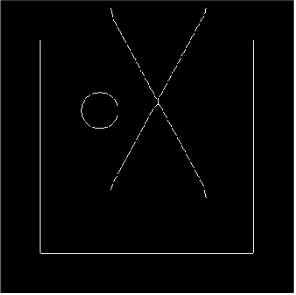
\includegraphics[width=.9\textwidth]{skeletonizeB}
\caption{Skeletonizada}
\end{subfigure}
\caption{Ejemplo de eskeletonize.}\label{fig:3.6}
\end{figure}


\section{Grafos}	
La teoría de grafos~\cite{Wiki:Grafos} en un campo dentro de la computación y de las matemáticas, estudia las propiedades de los grafos son utilizados para representar relaciones habitualmente, y están formados por:
\begin{itemize}
	\item Vértices o nodos: Que representan un objeto, persona o animal del entorno.
	\item Aristas o arcos: Que representan una relación o propiedad que comparten dos nodos, comunicándolos entre si.
Un ejemplo de dos nodos que forman un grafo estará mostrado a continuación en la figura~\ref{fig:3.7}.
\end{itemize}

Es una rama muy amplia pero solo vamos a centrarnos en uno de los problemas que podemos resolver gracias a estas teorías.
\begin{figure}[h]
\centering
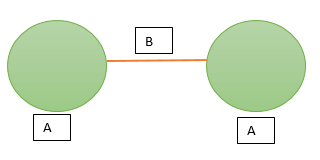
\includegraphics[width=.6\textwidth]{Grafo_Aris_y_Ver}
\caption{A): Son los vértices y B): Es una arista}
\label{fig:3.7}
\end{figure}

\subsection{K-componentes}
Es una de las propiedades del grafo, con sus componentes, nos indica cómo de fuertemente conexos están sus nodos o vértices.
Gracias a esta teoría, aprovechamos para afirmar, que cuando un grafo esta dividido en clusters, agrupaciones fuertemente conexas de parte de sus vértices.
Por el problema de los k-componentes, podemos saber que conjuntos de vértices forman los clusters, por lo tanto, aplicado a nuestro problema.
Los vértices que tengan aristas que los comuniquen, pertenecerán a las mismas rectas y de cada conjunto de vértices, sacaremos una recta.

\section{Bordes}
En lo que nos estamos basando, para poder resolver el problema,
es en la detección de bordes mediante kernels conocidos.
Para poder detectar donde esta el cambio de color en el histograma y esos cambios bruscos de pigmentación son los que nos indican que eso es un borde.
Para ello se han desarrollado numerosos métodos matemáticos, que pasando una máscara por toda la imagen, nos devuelven otra imagen con los bordes llamada máscara.

En los anexos se encuentra detallado cada uno de ellos, por lo que en adelante sólo nos limitaremos a listarlos.

Kernel \cite{wiki:kernels} \footnote{Dos párrafos mas arriba se usa un Kernel para las operaciones.} Un kernel es una matriz que se operara con una porción de pixeles para suavizar o detectar algún elemento que sea de nuestro interés.

Laplace~\cite{wiki:Laplace}, Prewitt~\cite{wiki:Prewitt}, Scharr~\cite{jon:Scharr}, Sobel~\cite{wiki:Sobel}, Roberts~\cite{wiki:Roberts}, Kirsch~\cite{wiki:Kirsch}, Gabor~\cite{wiki:Gabor}.
 
Aparte de los métodos antes mencionados hemos combinado distintos formas para detectar bordes através de los autovectores \cite{wiki:Eigenvector} largos, de la matriz Hessiana \cite{wiki:Hessiana}.
\capitulo{4}{Técnicas y herramientas}

Esta parte de la memoria tiene como objetivo presentar las técnicas metodológicas y las herramientas de desarrollo que se han utilizado para llevar a cabo el proyecto. Si se han estudiado diferentes alternativas de metodologías, herramientas, bibliotecas se puede hacer un resumen de los aspectos más destacados de cada alternativa, incluyendo comparativas entre las distintas opciones y una justificación de las elecciones realizadas. 
No se pretende que este apartado se convierta en un capítulo de un libro dedicado a cada una de las alternativas, sino comentar los aspectos más destacados de cada opción, con un repaso somero a los fundamentos esenciales y referencias bibliográficas para que el lector pueda ampliar su conocimiento sobre el tema.



\capitulo{5}{Aspectos relevantes del desarrollo del proyecto}

\section{Entorno de desarrollo}
Como entorno de desarrollo de los prototipos hemos utilizado Jupyter, ya que en sus notebooks interactivos puedes ejecutar directamente código Python como si fuese un intérprete.
Y Eclipse mas PyDev, como IDE, para programar en clases y paquetes de forma mas cómoda.
\subsection{Ventajas}
\begin{itemize}
\item He podido añadir widgets para calibrar en buen grado las funciones que hemos utilizado.
Gracias a estos widgets podemos dar valores e ir viendo como cambia la salida de la función de forma interactiva. Como podemos observar en la imagen \ref{fig:5.1}.

\begin{figure}[h]
\centering
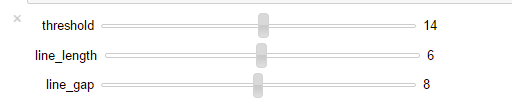
\includegraphics[width=0.65\textwidth]{Widget}
\caption{Ejemplo de un widget sobre la función de Hough}
\label{fig:5.1}
\end{figure}

\item Su rápida visualización sin tener grandes conocimientos de interfaz gráfica ha sido un gran apoyo para poder visualizar desde el principio las imágenes procesadas y como quedaban. Como podemos observar en la imagen \ref{fig:5.2}. 

\begin{figure}
\begin{subfigure}[b]{.5\linewidth}
\centering\large 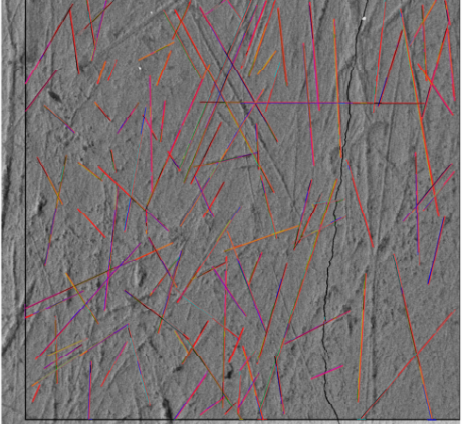
\includegraphics[width=.9\textwidth]{ComparativaLineas2}
\caption{Líneas antes de unir}
\end{subfigure}%
\begin{subfigure}[b]{.5\linewidth}
\centering\large 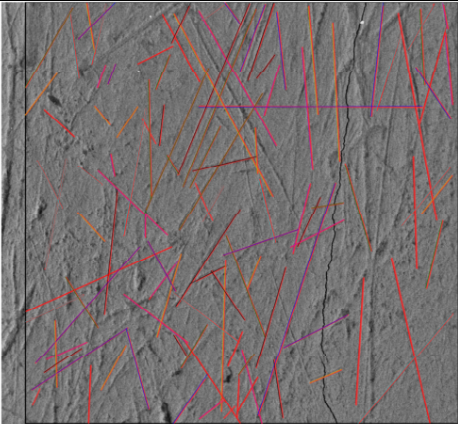
\includegraphics[width=.9\textwidth]{ComparativaLineas1}
\caption{Líneas después de unir}
\end{subfigure}
\caption{Ejemplo de una visualización del resultado intermedio de las funciones.}\label{fig:5.2}
\end{figure}


\item Desde el propio entorno puedes ejecutar, no solo código estructurado en script, sino también código estructurado en clases y llamadas a métodos es como un IDE pero con limitaciones. Como podemos observar en la imagen \ref{fig:5.3}.

\begin{figure}[h]
\centering
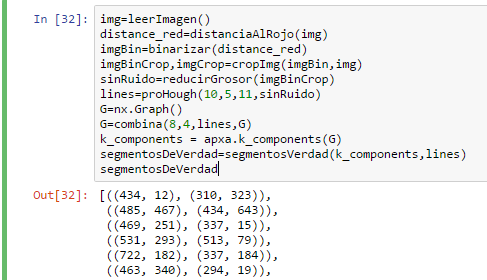
\includegraphics[width=0.65\textwidth]{Ejecucion}
\caption{Ejemplo de una ejecución.}
\label{fig:5.3}
\end{figure}

\item Multitud de librerías y funciones que en entornos parecidos como Matlab serian de pago y aquí al ser software libre el ejemplo anterior lo resume en una librería Numpy \cite{Numpy}.
\end{itemize}

\section{Procesado imagen}
Para llegar a conseguir calcular las líneas que había pintadas en las imágenes, tube que realizar una serie de pasos que vamos a resumir en tres etapas.
\subsection{Binarización}
Partiendo de una imagen que solo tenía líneas en rojo pintadas encima de las estrías producidas por el desgaste y lo demás de la imagen en escala de grises. Lo primero fue leer la imagen a trabes de las funciones ya programadas en la librería de Scikit-Image(skimage) \cite{scik:skeleton}.
Una vez que tenemos la imagen guardada en el espacio de color RGB podemos empezar el procesado quedándonos con el canal Rojo.

Calculamos la distancia de cada pixel de la imagen al color deseado, pasamos la imagen de distancias a blanco y negro y así tendremos un valor entre 0 y 256 en cada pixel correspondiente a la distancia al color. Cuanto mas alejado mas negro y los que sean del color, en blanco.

Para que la diferencia sea blanco o negro binarizamos, la imagen con un valor umbral así los valores de la distancia que sean mayores que el umbral pasaran a valer máximo y los que no consigan pasar el umbral serán los bordes blancos \ref{fig:5.4}.


\begin{figure}
\begin{subfigure}[c]{.5\linewidth}
\centering\large 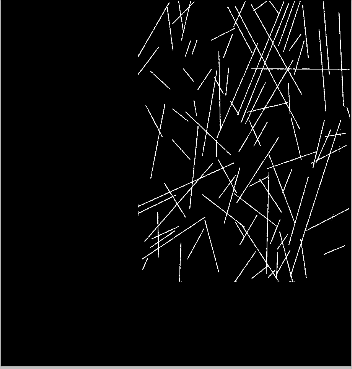
\includegraphics[width=.9\textwidth]{paso1Binariza}
\caption{Original}
\end{subfigure}%
\begin{subfigure}[c]{.5\linewidth}
\centering\large 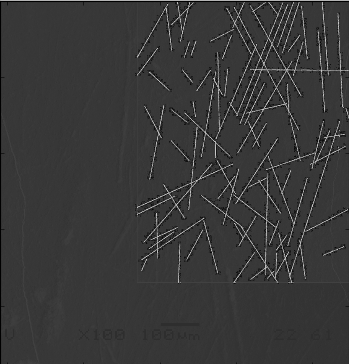
\includegraphics[width=.9\textwidth]{paso1DistanciaR}
\caption{Distancia al rojo}
\end{subfigure}
\begin{subfigure}[c]{.5\linewidth}
\centering\large 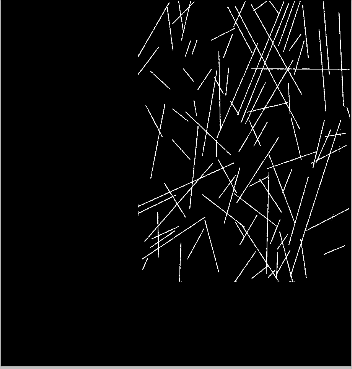
\includegraphics[width=.9\textwidth]{paso1Binariza}
\caption{Imagen binarizada}
\end{subfigure}
\caption{Resumen visual binarización.}\label{fig:5.4}
\end{figure}


\subsection{Obtener segmentos}
Partimos de la imagen binarizada y lo primero es reducir el grosor de las líneas detectadas a un pixel, eso lo conseguimos llamando a la función skeletonize que nos devuelve la imagen con las líneas de un pixel (así no acumulamos errores y es mas rápida la búsqueda de rectas).\\
Seguidamente llamamos a la función <<probabilistic hough line>> que nos va a encontrar segmentos que formaran las líneas el funcionamiento ha sido explicado en el apartado (conceptos teóricos). Como podemos observar en la figura \ref{fig:5.5}.


\begin{figure}
\begin{subfigure}[c]{.5\linewidth}
\centering\large 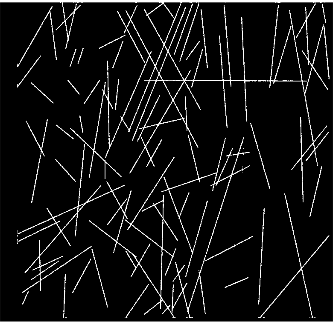
\includegraphics[width=.9\textwidth]{paso2Binaria}
\caption{Binarizada}
\end{subfigure}%
\begin{subfigure}[c]{.5\linewidth}
\centering\large 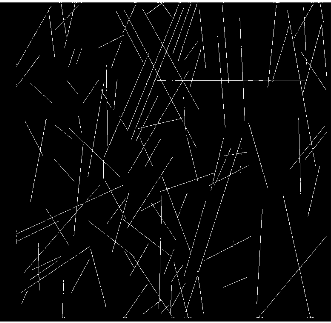
\includegraphics[width=.9\textwidth]{Paso2Skele}
\caption{líneas a 1 pixel}
\end{subfigure}
\begin{subfigure}[c]{.5\linewidth}
\centering\large 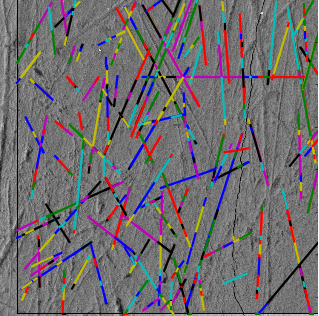
\includegraphics[width=.9\textwidth]{Paso2Segmentos}
\caption{Imagen original con segmentos}
\end{subfigure}
\caption{Resumen visual Obtener Segmentos.}\label{fig:5.5}
\end{figure}

\subsection{Procesado de segmentos}
Llegados a este punto, lo que tenemos son:
\begin{itemize}
\item Muchos segmentos que forman las líneas reales y tenemos que unirlos. Para ello vamos a usar la teoría de grafos añadiendo los segmentos a un grafo.

\item Para unir dos segmentos tiene que cumplirse que la distancia mínima entre sus extremos sea menor que un umbral y si pasa este punto comprobaremos que el angulo que forman entre ellas sea menor a otro umbral.

\item Si cumplen las dos condiciones añadiremos un camino al grafo desde la recta uno a la recta dos como se ve en la figura \ref{fig:5.6}.
\end{itemize}


\begin{figure}
\begin{subfigure}[b]{.5\linewidth}
\centering\large 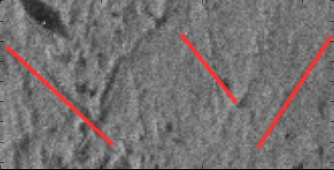
\includegraphics[width=.9\textwidth]{grafoLineasOri}
\caption{Imagen con segmentos en rojo.}
\end{subfigure}
\begin{subfigure}[b]{.5\linewidth}
\centering\large 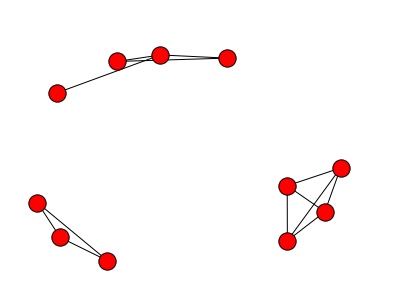
\includegraphics[width=.9\textwidth]{grafo}
\caption{Grafo de clusters de segmentos.}
\end{subfigure}
\caption{Resumen visual procesado de Segmentos.}\label{fig:5.6}
\end{figure}

\subsection{Recuperación de líneas}
Ahora lo que tenemos es un grafo con clusters, ya que cada cluster se identifica con únicamente una recta y tendremos tantos como rectas.
Un problema de grafos es el problema de las k-componentes pero a nosotros solo nos interesan las 1-componentes del grafo ya que cada grupo de estos segmentos cercanos se corresponde con una recta real.
Devolvemos la combinación de los segmentos mas relevantes de cada cluster y estos se convierten en nuestra buscada linea real \ref{fig:5.7}.
\begin{figure}[h]
\centering
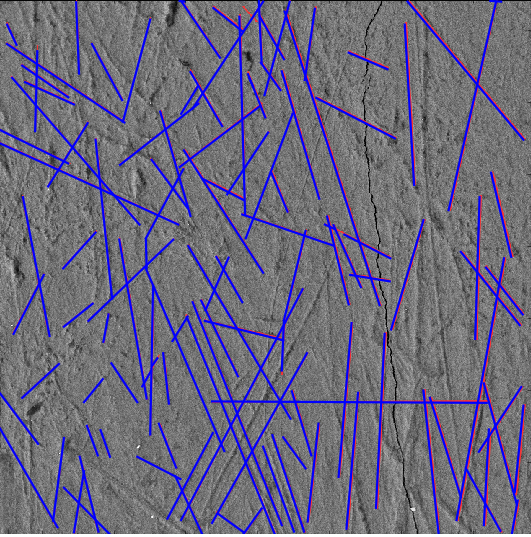
\includegraphics[width=0.65\textwidth]{ResultanteDelGrafo}
\caption{Líneas obtenidas después de procesar el grafo}
\label{fig:5.7}
\end{figure}

\subsection{Resumen pasos}

\begin{itemize}
\item Binarizar la imagen para solo quedarnos con los objetos de interés
\item Obtener segmentos que forman trozos de las líneas.
\item Añadir caminos entre las líneas cercanas en un grafo.
\item Obtener los grupos de líneas próximas y devolver la recta que las una. 
\end{itemize}

\section{Interfaz}
La programación de interfaces en Python ha sido bastante sencillo y muy intuitiva, por lo que lo recomendamos para futuras ocasiones.

En grandes rasgos estoy bastante contento con PyQt5 me ha resultado muy útil y la librería de Matplotlib también ya que con ellas he conseguido resolver todos los problemas planteados.


\capitulo{6}{Trabajos relacionados}

En esta sección, vamos a hablar de otros trabajos que están relacionados, tanto en la resolución del problema nuestro en particular, como resolver el problema de las detecciones de otro tipo de estrías o información.

\section{Paper de Alejandro Pérez Pérez:}
El articulo \cite{perez:perez}, es en que se basan en todos los artículos que hay hasta el momento para resolver este problema, lo mencionamos por esta importancia.

En este articulo se habla de como a partir de las micro estrías bucales, observadas al microscopio, podemos ver los distintos patrones que estas crean, diferentes dependiendo de la dieta que se llevara, una vez analizadas medidas y clasificadas mediante las formulas que proponen podemos clasificarlos en las distintas áreas que cada uno de las clasificaciones genera.

\section{Paper de Rebeca García González}
El articulo \cite{Rebeca:garcia} de nuestro cliente en el que analiza un ejemplo para datar la dieta correspondiente.

\section{Trabajo fin de grado: Sergio Chico Carrancio}
Podemos acceder al proyecto de Sergio en : \url{https://github.com/Serux/perikymata}.
En este proyecto se centraron en detectar estrías, pero no eran las mismas que nosotros queremos detectar, sino unas estrías llamadas perykimatas, estas muestran el crecimiento del diente. Pero muchas de las funcionalidades y partes del programa, son parecidas a las nuestras, aunque solucionado de formas distintas.

\capitulo{7}{Conclusiones y Líneas de trabajo futuras}

Todo proyecto debe incluir las conclusiones que se derivan de su desarrollo. Éstas pueden ser de diferente índole, dependiendo de la tipología del proyecto, pero normalmente van a estar presentes un conjunto de conclusiones relacionadas con los resultados del proyecto y un conjunto de conclusiones técnicas. 
Además, resulta muy útil realizar un informe crítico indicando cómo se puede mejorar el proyecto, o cómo se puede continuar trabajando en la línea del proyecto realizado. 



\section{Conclusiones:}
Para desarrollar este punto las vamos a ir separando por puntos dependiendo de la temática y de los campos a los que se refieran.
Pero van a ir cubriendo todas las conclusiones a las que hemos llegado, cubriendo todos los puntos mas relevantes que hemos realizado.

\begin{itemize}
\item Dinámica del proyecto: Para concluir con el proyecto, estoy muy satisfecho con la dinámica del proyecto, y con todos los aspectos que hemos tocado dentro del mismo.
Algunos aspectos de investigación han sido difíciles, no hay demasiada información respecto al tema, y somos los primeros en hacer una aplicación para resolver estos problemas, por lo que nos hemos encontrado aveces con impedimentos que hemos solucionado invirtiendo mas tiempo.

\item Transparencia al usuario: El reto mas grande ha sido conseguir realizar todas las funciones, con la mas sencilla transparencia para el usuario, ante todo hemos invertido parte del tiempo, no solo en resolver sino en pensar cual seria la forma mas sencilla, para que un usuario use el programa intuitivamente. 
\item Procesado y extracción de características: Los algoritmos para el procesado y la reconstrucción de las características que necesitábamos obtener, no eran directos. Como la variabilidad de tantos parámetros afectaba enormemente al resultado final, hemos tenido que ir testando muchos valores, para al final generalizarlos y conseguir un resultado bueno.

\item Uso del conocimiento adquirido durante la carrera: Durante el proceso de desarrollo hemos echo uso de muchos conceptos disjuntos que hemos dado durante la carrera y juntándolos para conseguir nuestras necesidades.

\item Lenguaje de desarrollo: El lenguaje de desarrollo, Python, es un plus para el proyecto ya que al investigar sobre este, hemos visto que últimamente en investigación y procedimientos matemáticos esta al alza, dispone de una gran cantidad de librerías con funciones muy actuales y de fácil aplicación. La programación es mas eficiente que en otros lenguajes.

\item Agilidad: Para completar este punto nosotros hemos tenido una curva de desarrollo muy estable y muy alta, ya que nos hemos centrado exclusivamente a este proyecto.
Por otra parte como agilidad en lo referido a metodología de desarrollo Scrum \cite{Scrum}, ha sido muy útil, porque en cada Sprint teníamos, una version con algunas capacidades añadidas, pero usable desde el primer momento.

\item Valor adquirido por mi: 
El principal motivo para la elección de este proyecto fue, el tema del mismo, es algo que si no se hace en colaboración con una universidad no es muy probable que surja, otro de los motivos fue el propio campo de la antropología, es algo que siempre me ha gustado y nunca tuve la oportunidad de conocer mas a fondo.
También como lenguajes de desarrollo elegí Python, porque en este lenguaje no sabia como hacer interfaces gráficas y como lo hemos dado en varias asignaturas quería terminarlo de completar sabiendo usar las interfaces ya que en contraposición en Java si que he visto y tocado en varias ocasiones el desarrollo de interfaces.

\item Los patrones de diseño:
Después de hacer este proyecto y las dificultades que han surgido, me he dado cuenta que las asignaturas de diseño debería de haberlas cursado, porque me han resuelto muchos problemas y me han ahorrado mucho tiempo.
Pero no viene de mal mencionar que al final las he usado y las he aprendido porque he querido completar mi formación.


\end{itemize}



\section{Líneas de trabajo futuras:}
Como partes de mejora futuras podríamos enumerar varios aspectos del proyecto.

\begin{itemize}
	\item Detección automática de bordes: 
Podríamos proponer a incluir, un algoritmo mas especializado en la detección de bordes, ya que las limitaciones que nos hemos encontrado hacen que este sea el puto mas flojo del proyecto, como propuesta, podría ser la creación desde cero de un algoritmo que detectase los bordes de una manera mas precisa.

	\item Unión de segmentos: 
La transformada de Hough para la detección de las lineas ha dado muy buenos resultados pero creo que se podría mejorar con este algoritmo: 

	\begin{itemize}
		\item Binarizar como hasta ahora.
		\item Esqueletonizar la imagen como hasta ahora
		\item Detectar las lineas mas grandes en la imagen y borrarlas de la mascara.
		\item Detectas las lineas bastante mas pequeñas pero aun no la mas cortas del todo y borrarlas de la mascara.
		\item detectar las lineas cortas en la imagen y borrarlas de la mascara
		\item Filtrar las lineas que en la mascara no contengan mas de un 70 por ciento de blanco así quitamos falsos positivos.
	\end{itemize}
	\item Añadir mas tipos de estrías que podríamos detectar como modos auxiliares para determinar que características queremos extraer de la imagen. Es decir acoplar en la aplicación la resolución de un nuevo problema de detección.
	
\end{itemize}


\bibliographystyle{plain}
\bibliography{bibliografia}

\end{document}